\section{Singlet and Triplet Excited States}
\label{sec:excitedStates}

\begin{center}
    \captionsetup{type = figure}
    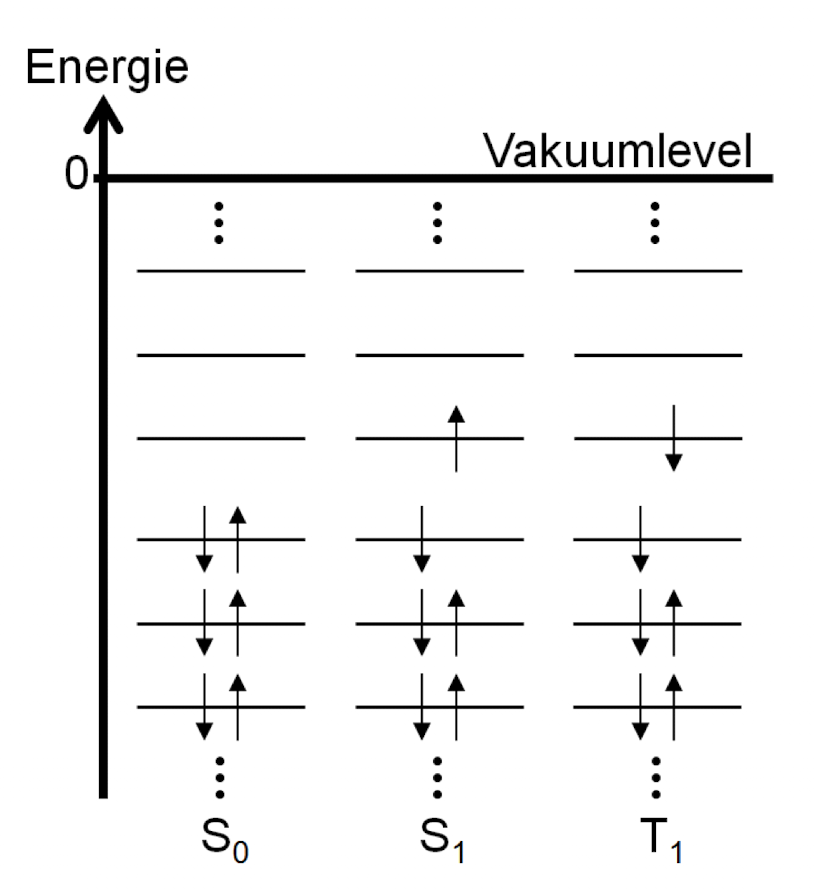
\includegraphics[width = 0.4\textwidth]{Pictures/Excited-States.png}
    \captionof{figure}{
        Orbital diagram of the dominant orbital occupations of the singlet states $S_0$ , $S_1$ and the triplet state $T_1$. \cite{Kilchert.04.2023} 
    }
    \label{fig:states}
\end{center}

In this section we want to discuss the relevant aspects of electronic processes in organic molecules. The energy levels of these systemes can be described by molecular orbitals. Molecular orbitals can be obtained through the usage of the \textbf{LCAO} method, which combines multiple atomic orbitals to a molecular orbital. A concrete occupation if these orbitals is called state, which have two specific states called \textbf{HOMO} (Highest Occupied Molecular Orbital) and \textbf{LOMO} (Lowest unOccupied Molecular Orbital). In addition to that distinction is made between singlet and triplet state with the following properties
\begin{itemize}
    \item Triplet State $T_i$: Total spin (sum of all electron spins) is $\pm 1$, 
    \item Singlet State $S_i$: Total spin is 0.
\end{itemize}
Figure \ref{fig:states} shows a simplified representation (only the largest contribution) of electronic states in molecules. 

\begin{center}
    \captionsetup{type = figure}
    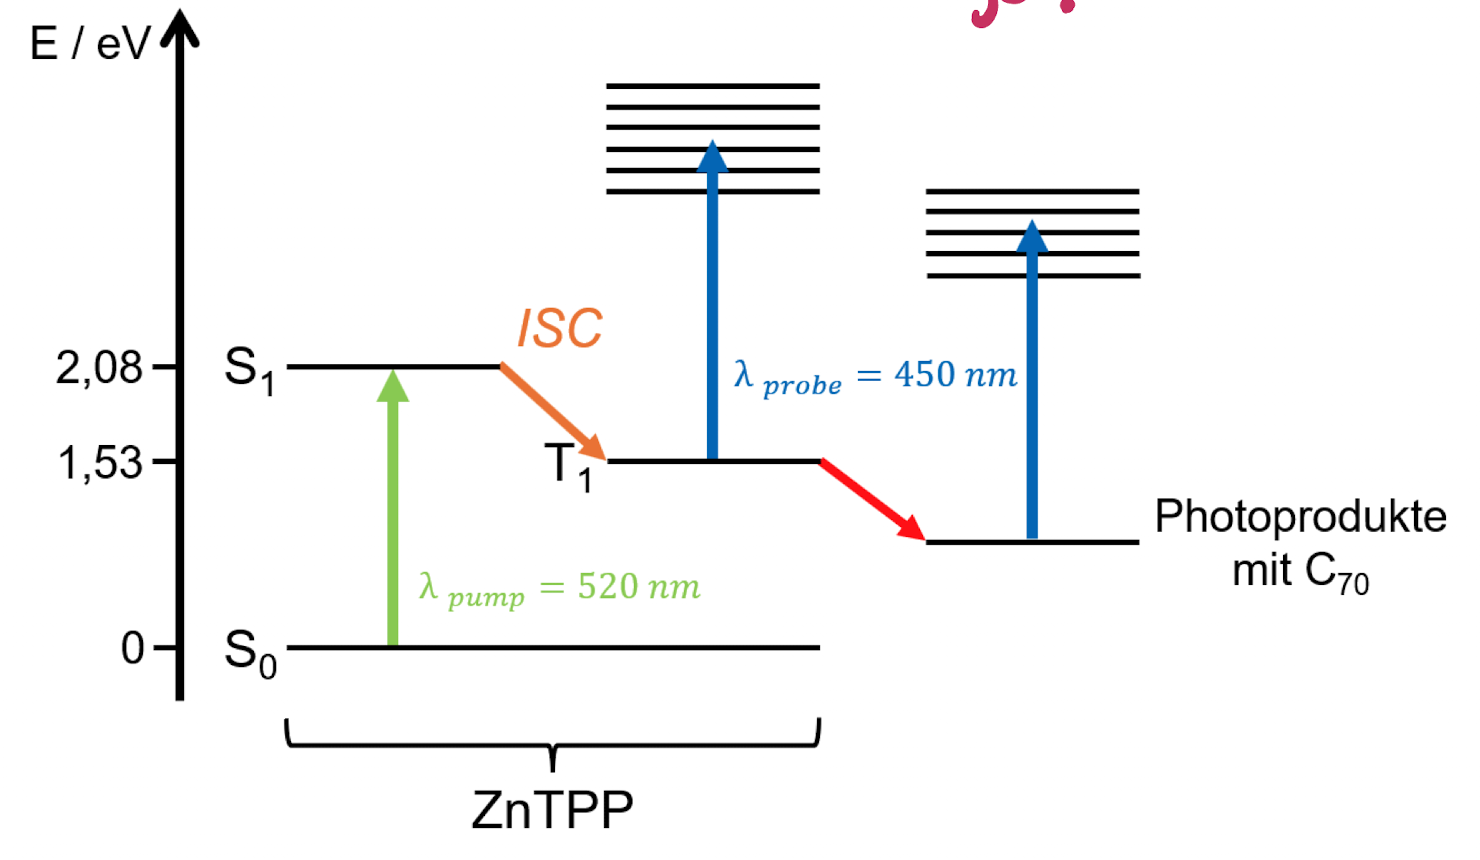
\includegraphics[width = 0.6\textwidth]{Pictures/Transition.png}
    \captionof{figure}{
        Jablonski scheme of the system of this experiment (ZnTPP and ZnTPP with fullerene $\mathrm{C}_{70}$). \cite{Kilchert.04.2023} 
    }
    \label{fig:transition}
\end{center}
To excite a system into from the ground state to the singlet state the system has to absorbe a photon with the energy corresponding to the transition, which leads to an absorption pattern the refelcts the structure of the energy levels of an atom. After absorption the electron relaxes back into the ground state (\textit{Kasha's Rule}). The transition can be radiative or non-radiative, but it is also possible to perform a transfer to a triplet state if the energy gap is small enough and one spin is flipped, which results in a sufficiently large spin-orbit coupling. The transition between singlet to triplet states is called Inter System Crossing (ISC). The jablonski scheme of this transition process for the relevant molecule of this experiment (ZnTPP and ZnTPP with fullerene $\mathrm{C}_{70}$) is shown in Figure \ref{fig:transition}. 
\bigskip

The radiative transition of an electron from the singlet state to the ground state is called \textbf{Flourescence} and from a triplet state to the ground state \textbf{Phosphorescence}. Both mentioned transitions are examples for \textit{radiative decays} with the emission of a photon. In case of ISC it is a \textit{non-radiative decay}, since the energy of the excited singlet state gets disspated due to ISC. The lifetime $\tau$ of the excited state will be given by the expression
\begin{gather}
    \tau = \frac{1}{k_\mathrm{r} + k_\mathrm{nr}},
\end{gather}
with the $k_\mathrm{r}$ and $k_\mathrm{nr}$ as the decay rates of the radiative and non-radiative decay. The determination is achieved by a pump-probe experiment, which will be discussed in Chapter \ref{sec:transient}. \cite{Kilchert.04.2023}
Scince the process of ISC is non-radiative one can not directly measure ISC, but if the energy level aif the singlet state is known and the decay rate of the triplet state will be measured, it is possible to indirectly measure the energy loss of ISC.